
%(BEGIN_QUESTION)
% Copyright 2010, Tony R. Kuphaldt, released under the Creative Commons Attribution License (v 1.0)
% This means you may do almost anything with this work of mine, so long as you give me proper credit

{\it Distillation} is a process of continuous boiling and condensing used to separate mixtures of different fluids.  A practical example of distillation is the separation of crude oil into multiple gases and liquids (propane, butane, naphtha, hexane, etc.).  Components with higher boiling points (typically denser fluids) collect at the bottom of the tower, while components with lower boiling points (typically lighter fluids) and gases collect at the top of the tower.

In this distillation tower, the level of liquid product at the bottom is sensed by a displacer-style level transmitter:

$$\includegraphics[width=15.5cm]{i00269x01.eps}$$

An instrument technician calculates the buoyant force for the displacer of this level instrument to be 0 pounds at 0\% liquid level, and 3.75 pounds at 100\% liquid level.  Explain how you would check the calibration of this instrument while the distillation tower was running, using these figures.

\vskip 20pt \vbox{\hrule \hbox{\strut \vrule{} {\bf Suggestions for Socratic discussion} \vrule} \hrule}

\begin{itemize}
\item{} What safety concerns are there in this process that you would have to be aware of?
\item{} What {\it standard} will you use for calibration (i.e. the thing you check the instrument's calibration against)?
\item{} Are there any process-related factors that could skew the calibration accuracy of this instrument while it is in service?
\end{itemize}

\underbar{file i00269}
%(END_QUESTION)





%(BEGIN_ANSWER)

Don't forget to contact the operator(s) for this process, and either have that operator put the level controller in manual mode, or you do it yourself!  The distillation tower bottom product level will have to be manually controlled for the duration of your calibration test.

%(END_ANSWER)





%(BEGIN_NOTES)

Two major options exist here: {\it wet} calibration or {\it dry} calibration.  In either case, the operator needs to first place the level controller in manual mode so that your calibration work doesn't cause the level control valve to move all over the place, messing up the actual column bottoms level.

\vskip 10pt

For a wet calibration, empty the cage and check the LRV (zero).  Then, fill the cage full of bottoms product and check the URV.

\vskip 10pt

For a dry calibration, empty the cage and check the LRV (zero).  Then, apply 3.75 pounds up upward force to the displacer and check the URV.


\vfil \eject

An interesting lesson in professional ethics and safety related to displacer-type level instruments is an incident which happened at an oil refinery where I worked in 1989.  A Fisher Level-Trol pneumatic transmitter was sensing and controlling liquid butane level at the bottom of the ``debutanizer'' distillation tower in the refinery's crude unit.  During unit start-up, operators noticed a problem: their indication at the DCS console in the control room (coming from a P/I converter on the Level-Trol's output) showed a saturated-high level reading when the field operator verified 0\% level in the debutanizer tower looking at the sightglass (LG):

$$\includegraphics[width=15.5cm]{i00269x02.eps}$$

\vskip 10pt

\filbreak

Here is the sequence of events:

\begin{itemize}
\item{} Operators noticed the LIC reading 105\% level in the tower bottoms.
\item{} A field operator reads 0\% level in the LG on the same tower.
\item{} An instrument tech is summoned to repair the Level-Trol transmitter.  {\it What do you suppose could be wrong with it, to make it register falsely high?}
\item{} It is a cold winter night, and the technician decides the correct way to fix the problem is to turn the zero adjustment on the Level-Trol so that it now outputs a signal of 0\%, matching the sightglass.  {\it What is wrong with this action?}
\item{} The technician leaves to return to the warm shop, rather than verify that the transmitter continues to measure level correctly.
\item{} Unknown to the technician, the Level-Trol is actually broken: the displacer has fallen off the end of the torque tube level, leaving the torque tube unweighted.  This allows the torque tube to spring to its ``full'' position, which is what made it register 105\% in the first place.  Moving the zero calibration screw did absolutely nothing to fix the problem!
\item{} The LIC responds to the transmitter's 0\% signal by shutting the bottom product valve, accumulating liquid butane inside the tower.
\item{} As liquid butane accumulates inside the tower, the failed Level-Trol transmitter continues to read 0\%, and the LIC continues to hold the bottom product valve shut.
\item{} Liquid butane level accumulated until the LAH alarm sounds.  Operators acknowledge the alarm.
\item{} Liquid butane level accumulated until the LAHH alarm sounds.  Operators acknowledge this alarm too.
\item{} The tower eventually fills completely full of liquid butane, at which point the tower's contents become incompressible and the relief valve lifts.
\item{} As a cascade of liquid butane exits the relief valve, a pool of liquid butane accumulates on the ground surrounding the tower.  This continues for about a minute.
\item{} Something touches off the butane, and it erupts into flame.  The debutanizer tower and its open relief valve are on fire.  The flame exiting the relief valve is at least as tall as the tower itself.
\item{} Firefighters work to extinguish the blaze.  They are able to put out the fire before it causes any other vessel to overpressure.
\item{} Operators shut down the crude unit.  The unit is down for repair for over a month (at an operational loss of about \$1 million per day!).
\end{itemize}


\vskip 20pt \vbox{\hrule \hbox{\strut \vrule{} {\bf Suggestions for Socratic discussion} \vrule} \hrule}

\begin{itemize}
\item{} What did the technician do wrong?
\item{} If you were the technician, what would you have done differently?
\item{} What did the operators do wrong?
\item{} If you were one of the operators, what would you have done differently?
\end{itemize}

%INDEX% Measurement, level: displacer (buoyancy)
%INDEX% Process: distillation (generic)

%(END_NOTES)


